
%%%%%%%%%%%%%%%%%%%%%%% file typeinst.tex %%%%%%%%%%%%%%%%%%%%%%%%%
%
% This is the LaTeX source for the instructions to authors using
% the LaTeX document class 'llncs.cls' for contributions to
% the Lecture Notes in Computer Sciences series.
% http://www.springer.com/lncs       Springer Heidelberg 2006/05/04
%
% It may be used as a template for your own input - copy it
% to a new file with a new name and use it as the basis
% for your article.
%
% NB: the document class 'llncs' has its own and detailed documentation, see
% ftp://ftp.springer.de/data/pubftp/pub/tex/latex/llncs/latex2e/llncsdoc.pdf
%
%%%%%%%%%%%%%%%%%%%%%%%%%%%%%%%%%%%%%%%%%%%%%%%%%%%%%%%%%%%%%%%%%%%


\documentclass[runningheads,a4paper]{llncs}

\usepackage{amssymb}
\usepackage{amsmath}
\setcounter{tocdepth}{3}
\usepackage{graphicx}
\usepackage{tikz}
\usepackage{url}
\usepackage[linesnumbered,ruled]{algorithm2e}
\usepackage[toc,page]{appendix}
\usetikzlibrary{backgrounds,positioning}
\usetikzlibrary{decorations.pathreplacing}

\tikzset{
  cell/.style = {rectangle, draw, text width=1.3cm, outer sep=0pt},
  capx/.style = {rectangle, draw, text width=1.3cm, color=black!40,outer sep=0pt}
}

\usepackage{url}
\urldef{\mailsa}\path|{daniel.opitz, sebastian.graf, nikolai.baudis}@student.kit.edu|
\newcommand{\keywords}[1]{\par\addvspace\baselineskip
\noindent\keywordname\enspace\ignorespaces#1}

\begin{document}

\mainmatter  % start of an individual contribution

% first the title is needed
\title{Two Independent and Highly Efficient Open Source TKF91 Implementations}

% a short form should be given in case it is too long for the running head
\titlerunning{Efficient Open Source TKF91 Implementations}

% the name(s) of the author(s) follow(s) next
%
% NB: Chinese authors should write their first names(s) in front of
% their surnames. This ensures that the names appear correctly in
% the running heads and the author index.
%
\author{Nikolai Baudis \and Pierre Barbera \and Sebastian Graf \and  Sarah Lutteropp \and Daniel Opitz \and Tomas Flouri \and Alexandros Stamatakis}
%
%\authorrunning{Efficient Open Source TKF91 Implementations}
% (feature abused for this document to repeat the title also on left hand pages)

% the affiliations are given next; don't give your e-mail address
% unless you accept that it will be published
\institute{Karlsruhe Institute of Technology, Institute of Theoretical Informatics,\\
Kaiserstrasse. 12, 76131 Karlsruhe, Germany\\
\mailsa\\
\url{http://www.informatik.kit.edu/}}

%
% NB: a more complex sample for affiliations and the mapping to the
% corresponding authors can be found in the file "llncs.dem"
% (search for the string "\mainmatter" where a contribution starts).
% "llncs.dem" accompanies the document class "llncs.cls".
%

%\toctitle{Lecture Notes in Computer Science}
%\tocauthor{Authors' Instructions}
\maketitle


\begin{abstract}
In the context of a master level programming practical at the computer science department of the Karlsruhe Institute of Technology, 
we developed and make available two independent and highly optimized open-source implementations for the pair-wise 
statistical alignment model, also known as TKF91, that was developed by Thorne, Kishino, and Felsenstein in 1991. 
This paper has two parts. 
In the educational part, we cover teaching issues regarding the setup of the course and the practical and summarize student and teacher experiences. 
In the scientific part, the two student teams (Team I: Nikolai, Sebastian, Daniel; Team II: Sarah, Pierre) present their
solutions for implementing efficient and numerically stable implementations of the TKF91 algorithm. 
The two teams worked independently on implementing the same algorithm. Hence, since the implementations yield identical results ---with slight numerical deviations--- 
we are confident that the implementations are correct. We describe the optimizations applied and make them available as open-source codes 
in the hope that our findings and software will be useful to the community.

%In this documentation we describe our implementation of algorithmic DNA sequence alignment building on the TKF91 maximum likelihood evolutionary model. The goal of this project was to implement an application that computes the pairwise sequence alignment using the aforementioned model and that is highly optimized for performance. In order to maximize the performance, we utilized vectorization using SSE3 and AVX vector intrinsics. Further, we implemented optimizations such as an efficient memory layout, memoization, and address alignment, which all together keep overheads to a minimum. In addition, we ensured that our optimized program prevents numerical underflow.

%\keywords{Keywords}
\end{abstract}


\section{Introduction}
\label{sec:introduction}

In \cite{TKF91}, Thorne, Kishino, and Felsenstein presented a method for aligning DNA sequences using a maximum likelihood approach.
To this end, they developed an explicit statistical model of evolution that includes insertions, deletions, and substitutions of nucleotides 
as basic operations for comparing two DNA sequences. 
A given evolutionary model assigns a weight to each of these three basic operations.  
These are then used to design a dynamic programming algorithm that computes the maximum likelihood pair-wise alignment between two DNA sequences. 

As substitution model, we assume the standard stochastic nucleotide substitution model {\bf TODO by whom actually?}. 
{\bf TODO the other two?} 
The algorithm computes the optimal maximum likelihood sequence alignment using three matrices, one for each {\bf TODO}.
The algorithm is given by the following dynamic programming recurrence: 
\[
\begin{aligned}
  M^0(i,j)&=\frac{\lambda}{\mu}\pi_{a_i}\overline{p_0}(t)max\{M^0(i-1, j), M^1(i-1,j), M^2(i-1,j)\}\\
  M^1(i,j)&=\frac{\lambda}{\mu}\pi_{a_i}max\{P_{a_i \rightarrow b_j}(t) p_1(t), \pi_{b_j}\overline{p_1}(t)\}\\
          &\quad\quad max\{M^0(i-1, j-1), M^1(i-1,j-1), M^2(i-1,j-1)\}\\
  M^2(i,j)&=\pi_{b_j}\lambda\beta(t)max\{M^1(i,j-1), M^2(i,j-1)\}
\end{aligned}
\]
Where $\lambda$ and $\mu$ denote the birth and death rate, $\pi_x, x \in \{A,C,G,T\}$ denotes the equilibrium frequency of the nucleotides, 
$P_{x \rightarrow y}$ the transition probability from $x$ to $y$, and $\overline{p_n}(t)$ the probability that after time $t$ a mortal link has exactly $n$ descendants. 
The values for $t$, $\lambda$, $\mu$, and $\pi$ are given as input. 
The values for $\overline{p_n}$ can be pre-computed in constant time {\bf constant?}.

{\bf TODO related work} 

{\bf TODO acronyms: DP, DPM} 

The remainder of this paper is organized as follows: In Section~\ref{teaching}, we describe the teaching setup and goals. 
The teams then present their implementations in Sections~\ref{sec:implementation-1} and \ref{sec:implementation-2}, respectively. 
The corresponding experimental results by both teams are presented in Section~\ref{sec:evaluation}.
In the following Section~\ref{teaching-results}, we summarize our teaching experiences.
We conclude in Section~\ref{conclusion}.

\section{Teaching Perspective, Goals and Course Outline}
\label{teaching} 

\subsection{Teaching Setup \& Goals} 

Courses at the Master level in our computer science department are organized in so-called modules over two semesters.
In the first semester of the Bioinformatics module, we teach a lecture called ``Introduction to Bioinformatics for Computer Scientists'', since KIT does not offer
a stand-alone Bioinformatics degree. This lecture covers basic topics such as an introduction to molecular biology, pair-wise sequence alignment,
BLAST, de novo and by-reference sequence assembly, multiple sequence alignment, phylogenetic inference, MCMC methods, and population genetics.

In the second semester of the module, students can choose if they want to do a seminar presentation or the programming practical whose results we describe here.
The goal of the practical is to carry out a self-contained project and write, as well as release software, that is useful to the evolutionary biology community.
Another focus is on learning to use tools that enhance software quality.
Note that, at a CS department designing ``classic'' bioinformatics analysis pipelines using scripting languages is typically not considered as ``real programming'' by the
students. Hence, we needed to define a project that requires coding in \texttt{C/C++} or \texttt{Java}.
One should also strive to avoid having the students extend existing software, since
this is generally frustrating and hinders creativity.

We thus decided to ask the students to implement efficient, sequential versions of the TKF91 algorithm that can also be used as library routines. 
Since the dynamic programming algorithm as such, is relatively straight-forward to implement for a computer science student, the main focus was on code optimization. 
The students were thus asked to implement a highly efficient version of the code in \verb|C| or \verb|C++| using all capabilities of a modern CPU (e.g., SSE3 and AVX intrinsics).
The main motivation for this was to give the students enough time to experiment with low-level optimization strategies on modern CPUs. 
Moreover, this project allowed to apply a broad range of skills acquired in the Bioinformatics and other master-level modules at our department.
Furthermore, the TKF91 model required understanding and applying the discrete pair-wise sequence alignment methods and likelihood-based models for evolutionary biology 
presented in the lectures. 
To foster competition among the teams, an award (dinner payed by the PI) was announced for the team that would implement the fastest code. 
To allow for a fair comparison of the codes and CPU-specific optimization we provided the students access to a reference machine with 4 physical cores (Intel i7-2600 running at 3.40GHz) and 
16GB RAM. 

In terms of project documentation, students are usually required to write a report. However, in the present case, we jointly took the decision to write a paper 
about the practical and upload it to \verb|biorxiv|. This has the positive effect that students also learn how to write scientific papers.

\subsection{Code Quality Assessment}
In order to continuously monitor and improve the quality of our source code, we used several tools and methods throughout our project.
We deployed both, static, as well as dynamic code analyses.

\subsubsection{Static Analysis}
Static analyses help to identify static programming errors such as incorrect programming language syntax or static typing errors.
We compiled our code with the \texttt{gcc} compiler using all available and reasonable warning flags\footnote{-Wall -Wextra -Wredundant-decls -Wswitch-default -Wimport -Wno-int-to-pointer-cast -Wbad-function-cast -Wmissing-declarations -Wmissing-prototypes -Wnested-externs -Wstrict-prototypes -Wformat-nonliteral -Wundef}. 
This allowed us to identify potential programming errors at an early stage. 
Due to its more pedantic nature (i.e., ability to detect more errors), we also used the \texttt{clang} compiler with respective flags\footnote{-Weverything -pedantic} 
periodically alongside of \texttt{gcc} to further reduce the amount of potential errors.

\subsubsection{Dynamic Analysis}
These analyses cover run-time issues such as memory leaks.
We used \texttt{valgrind} and its sub-module \texttt{memcheck} for detecting memory-related errors in our programs. 


\section{Implementation of Team I}
\label{sec:implementation-1}

Before describing our vectorized implementation, we cover the necessary prerequisites.
In Section~\ref{ssec:dynprogramming} we describe the DP algorithm in more detail as well as the corresponding wave-front parallelism we exploited in our implementation. 
In Section~\ref{ssec:memorylayout}, we describe our memory layout concept, which is required to improve the efficiency of the vectorization. 
Thereafter, in Section~\ref{ssec:memo}, we describe how we cache intermediate computations, and then explain our vectorization approach in Section~\ref{ssec:vectorization}. 
In addition to that, Section~\ref{ssec:dataalignment} outlines our considerations regarding the alignment of the data, marking an important part of the vectorized implementation. 



\subsection{Dynamic Programming and Wave-front Parallelism}
\label{ssec:dynprogramming}

\textit{Dynamic Programming (DP)} is a widely-used technique to efficiently solve a class of, at first sight, apparently hard computational problems when they exhibit
\textit{overlapping subproblems} and \textit{optimal substructure}. 
Pair-wise sequence alignment falls into this class. 
Another advantage of DP is that it is comparatively straight-forward to parallelize computations along the anti-diagonals 
of the DP matrix. 
This DP matrix parallelization approach is also known as wave-front parallelism. 
The underlying idea is that matrix entries along the same DP anti-diagonal $d$ can be computed independently from each other  (and hence in parallel) 
if the preceding anti-diagonal $d-1$ has been computed. 
Therefore, we can deploy vector intrinsics to accelerate calculations along anti-diagonals.


\subsection{Memory Layout}
\label{ssec:memorylayout}

We first introduce our memory layout for the three DP matrices ($M^0, M^1, M^2$) since this is performance-critical.
Our vectorization approach needs to attain high data locality to take advantage of the CPU cache.
To this end,  we permuted the indexing scheme of the DP matrix such that matrix neighboring entries on a anti-diagonal are also contiguous in memory. 
Figure~\ref{fig:indexing} shows the memory mapping of the matrix. 
It is layed out neither in a column-major nor row-major fashion in memory, but stored linearly by anti-diagonals. 

\begin{figure}[ht!]
  \centering
  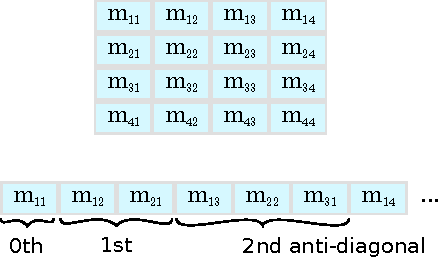
\includegraphics[scale=0.9]{figures/indexing.pdf}
  \caption{Memory layout for the DP matrix}
  \label{fig:indexing}
\end{figure}

We index the matrices using a modified version of the \textit{Cantor pairing function}, where a tuple is assigned to an offset. 
The original Cantor pairing function $\pi$ assigns an integer to a pair of integers (e.g., $\pi: (\mathbb{N}, \mathbb{N}) \rightarrow \mathbb{N}$). 
Since the size of the DPM is defined by the length of the input sequences and because it is not infinite, 
we modified the pairing function to accept a tuple of two integers from the interval $[0..\textrm{length}(\textrm{Sequence 1\textbar2})]$ as input. 
As a consequence, the DPM is divided into three parts: the \emph{opening}, \emph{middle}, and \emph{closing part}. 
In the opening part, the modified pairing function is identical to the original function; in the middle and closing parts, 
the modified pairing function is calculated by subtracting an offset from the original pairing function. 
We calculate the offset via the original Cantor pairing function.

\begin{figure}[ht!]
  \centering
  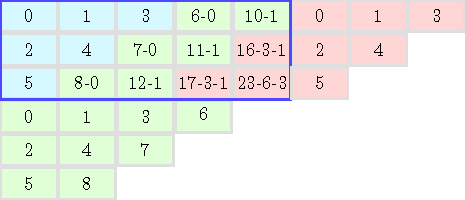
\includegraphics[scale=0.9]{figures/pairingfunc.pdf}
  \caption{Indexing scheme for the anti-diagonals}
  \label{fig:pairingfunc}
\end{figure}

In Figure~\ref{fig:pairingfunc}, we show the index calculations for the anti-diagonals of a $5\times3$-matrix. 
The blue border denotes the bounds {\bf ?} of the DP matrix, the blue cells represent the opening part, 
the green cells inside the matrix the middle, and the red cells inside the matrix the closing part. 
Green and red cells outside the matrix boundaries represent the Cantor pairing functions for the offset calculation for the middle and closing part, respectively. 
For this {\bf for what?}, only the first rows of those {\bf all?} pairing functions are needed. 

Given the anti-diagonal indexing scheme for a single matrix, we need to 
devise the memory layout for the three DP matrices ($M_0,M_1,M_2$) next.  
This is because, calculating a DP value requires 
accessing all three matrices.  
{\bf I am not sure I understand the following question, please re-formulate} Therefore, the access pattern inside the matrices follows the same anti-diagonals.  
To improve data locality while, at the same time, using efficient {\bf vector?} load and store operations, 
the matrix data has to be arranged accordingly.  
To this end, we evaluated the following three alternative matrix layouts (see Figure~\ref{fig:datalayout}):

\begin{figure}[ht!]
  \centering
  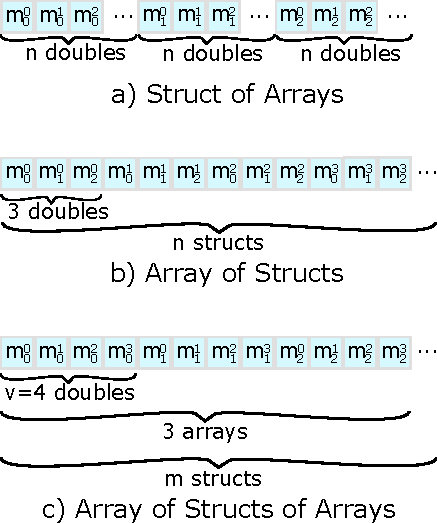
\includegraphics[scale=0.7]{figures/datalayout.pdf}
  \caption{Alternative data layouts for storing anti-diagonals}
  \label{fig:datalayout}
\end{figure}

\paragraph*{Struct of Arrays (SoA)} ({\small\texttt{struct \{ double m0[n], m1[n], m2[n]; \} data;}}) 
This layout allows for simple {\bf vector?} load and store patterns. 
However, the three matrices are located in separate memory regions, which decreases
cache efficiency and data locality.

\paragraph*{Array of Structs (AoS)} ({\small\texttt{struct \{ double m0, m1, m2; \}
data[n];}}) This layout exhibits improved data locality by grouping values
closely together that are -- in most cases -- accessed simultaneously. On the
other hand, loading and storing vectors requires disentangling and interleaving
them, which requires several, potentially costly, vector shuffle operations. 

\begin{figure}[ht!]
  \centering
  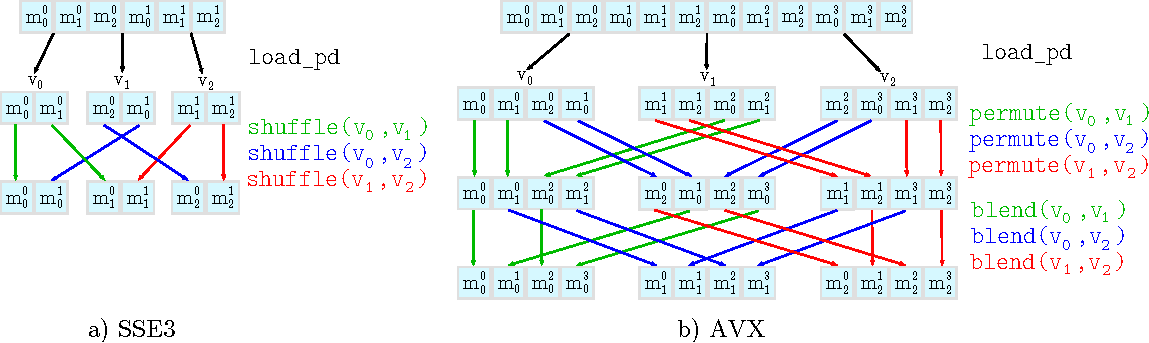
\includegraphics[scale=0.6]{figures/shuffle.pdf}
  \caption{Disentangling operations for a) SSE3 (128 bit) and b) AVX (256 bit) vectors.}
  \label{fig:shufflesse}
\end{figure}

Figure~\ref{fig:shufflesse} illustrates these shuffle operations. 
For $m_x^y$, the subscript $x$ indicates
the index of the matrix and the superscript $y$ the SSE3/AVX vector element index $y$ {\bf state that we use double precision!}.
The first row of the Figure depicts the {\em AoS} data layout. 
Here, we perform an (aligned {\bf if you say aligned you need to be more specific}) vector \texttt{load} operation 
to load the data into temporary vector registers. 
Thereafter, we shuffle the temporary vectors such that (i) each vector only contains elements from one of the tree DP matrices and 
(ii) the individual elements are in the correct order with respect to  the {\bf anti-?} diagonal. 
For both, SSE3 as well as AVX instructions we need to perform three \texttt{load} operations and three \texttt{shuffle}/\texttt{permute} operations. 
For AVX, we also require three \texttt{blend} operations to put the data elements into the correct order. 

\paragraph*{Array of Structs of Arrays (AoSoA)} ({\small\texttt{struct \{ double m0[v],
m1[v], m2[v]; \} data[m];}}) While this layout solves both of the previous problems {\bf state those problems again!},
grouping vectors {\bf what do you mean by grouping vectors?} in advance complicates DP cell access above the current anti-diagonal.
These values would {\bf would or do not lie?} not lie within vector boundaries and would {\bf would or do require?} then
again {\bf either?} require \texttt{shuffle}/\texttt{permute} operations or partial loads {\bf explain what you mean by partial loads!}.

\paragraph*{} All three layouts have different performance characteristics with respect to
cache efficiency {\bf Note to team I: we usually say cache efficiency and data locality, but not cache locality!} 
and complexity of the load, store, and shuffle operations.
We implemented prototypes for all three approaches to analyze their
performance and found that the AoS approach performs best.  
Note that, the complexity of the \texttt{shuffle} operations outweighed the improved cache efficiency in the AoS and
AoSoA layouts (also see Table~\ref{tbl:benchmark} in Section~\ref{}). 


\subsection{Memoization}
\label{ssec:memo}

The \cite{TKF91} model has several parameters. Thus, it initially seemed inevitable to carry out the non-trivial computations for filling DP cells 
for each cell from scratch.
However, after analyzing which expressions are constant and can thus be pre-computed and reused (i.e., memoized {\bf Note: this could also be called caching or using a lookup table}), 
we reduced the operations required for calculating a DP cell value to just three: indirection, summation, maximum.

Obvious savings can be achieved for expressions that only depend on the time parameter $t$, 
the birth rate $\lambda$, and the death rate $\mu$.
These values are constant and given as input parameters. 
We also observed that the cell updates in the DP algorithm only require a constant number of common sub-calculations/components: 
When the nucleotide values at the current indices in the two sequences are available, 
the score (cell value) can be computed using only the current nucleotide pair and the 
neighboring values {\bf of which matrices} in the dynamic programming matrix.

The memoization scheme (lookup table) for all possible transition penalties is shown in Figure~\ref{fig:memo}. 
The penalties $C^i$ take one or two nucleotides as parameters.
Thus they can be stored in a memoization table of $4$ and $16$ entries, respectively. 
With a total of only $24$ memoized values, we substantially simplified and accelerated (by {\bf TODO how many orders of magnitude?}) the cell updates.
In addition, this simplification now allows to apply the logarithm for preventing numerical underflow.
This was not possible before, since taking the logarithm of the original equation would have been too expensive. 
It also kept the translation to SIMD-enabled code manageable {\bf what do you mean by manageable?}.
Furthermore, the simplification reduces the number of design decisions that are required regarding 
memory layout and vectorization.

At a later point of the project, it became evident that the indexed loads from memoized penalty matrices caused a performance degradation. 
To solve this problem, we pre-compute a larger lookup table of vector-sized elements, that we index by a specific nucleotide permutation. 
Consider the following example for AVX vector intrinsics.
We need to calculate a bijective mapping for a set of four nucleotides to an integer representing one of the $4^4 = 256$ possible permutations (e.g., a perfect hash) 
for $C^0$ and $C^2$, and $4^{2 \cdot 4} = 65536$ for $C^1$ respectively {\bf where do those C variables come fraom, have they been properly introduced? I don't think so!}. 
The mapping is implemented as a base conversion from the set of 4 nucleotides to an unsigned integer via a appropriate bit-wise operations.

While this approach has exponential space requirements as a function of the vector width, using a lookup table of $65536 \cdot 32$ bytes $= 2$ MB for $C^1$ for 
the AVX version of our code was still feasible. 
However, the evaluation of the resulting performance revealed that too much time is spent to fill the table, at least for our benchmark datasets. 
Since the values in the table only depend on the likelihood model parameters, that is, it is independent of the input sequences at hand, 
this approach can be re-considered in cases were this lookup table shall be re-used for multiple DP invocations. 
This might be useful when calculating pair-wise alignments of $n$ sequences under the same model parameters 
{\bf not sure if we should write this here, at leats as long as the parameter t is also required to calculate the values in that table, need to double-check}
{\bf I don't understand the following sentence, please re-forumulate it} The scaling to wider vector registers could be retained by loading a register in packs of four values.

\begin{figure}
\[
\begin{aligned}
  C^0(a)&=\frac{\lambda}{\mu}\pi_{a}\overline{p_0}(t)\\
  C^1(a, b)&=\frac{\lambda}{\mu}\pi_{a}max\{P_{a \rightarrow b}(t) p_1(t), \pi_{b}\overline{p_1}(t)\}\\
  C^2(b)&=\pi_{b}\lambda\beta(t)\\
  M^0(i,j)&=C^0(a_i)max\{M^0(i-1, j), M^1(i-1,j), M^2(i-1,j)\}\\
  M^1(i,j)&=C^1(a_i,b_j)max\{M^0(i-1, j-1), M^1(i-1,j-1), M^2(i-1,j-1)\}\\
  M^2(i,j)&=C^2(b_j)max\{M^1(i,j-1), M^2(i,j-1)\}
\end{aligned}
\]
\caption{A re-formulation of the DP step using the memoized sub-problems $C^i$ {\bf you should have explained what the C is much earlier!}}
\label{fig:memo}
\end{figure}


\subsection{Vectorization}
\label{ssec:vectorization}

We implemented a vectorized version for computing 
$M_0$, $M_1$, and $M_2$ using \texttt{add}, \texttt{max}, \texttt{load}, and \texttt{store}
operations for both SSE3 and AVX instructions.  
Using these operations, we can process $n$ matrix elements in parallel.  
Depending on the location of the vector on the anti-diagonal that is being processed, there will be $0 < n \leq V$ valid elements to operate on 
per vector (with vector size $V = 4$ for AVX and $V = 2$ for SSE3 {\bf TODO: we need to state in the beginning that we used double precision}). 

Although we ensured aligned {\bf need to be more specific what you mean by aligned, it's not clear to a general readership} 
access to a majority of the data (as will be explained in
Section~\ref{ssec:dataalignment}), we used the unaligned vector \texttt{load} and \texttt{store}
operations \texttt{loadu\_pd} and \texttt{storeu\_pd} for the SSE3 and AVX versions. 
{\bf I don't get the following sentence, whyt was unaligned load necessary if you were able to test on aligned data???} 
This does not represent a disadvantage for the
performance, since we could not identify significant performance impacts of
using unaligned intrinsics on aligned data.

To prevent our \texttt{store} operations from overwriting data at the boundaries
of the matrices, we ensured that for vectors with size $n < V$ (i.e.,
not completely filled/padded vectors) only $n$ elements are written back into the
matrices.  For the SSE3 version, this can be achieved by only writing the lower
part of the vector if its size is $1$.  For AVX, however, we covered all cases
where $n < V$ holds using the \texttt{maskstore\_pd} intrinsic and an appropriate mask
for all possibles value of $n$ (i.e., $3$, $2$, and $1$).

\subsection{Data Alignment}
\label{ssec:dataalignment}

When vectorizing along the anti-diagonals, accessing the memory in the dynamic programming matrices when they are stored in a row-, or column-major scheme 
prevents deploying efficient vector operations for loading the values from the matrices into vector registers. 
For such a memory layout, the performance of the inner DP loop becomes heavily memory-bound. 
Therefore, we used the aforementioned memory layout {\bf TODO: add cross-ref}, such that \texttt{load} and \texttt{store} operations for copying data directly from the anti-diagonal 
into vector registers can be utilized. 
Those \texttt{load} and \texttt{store} operations come in two flavors: There exist \texttt{load} and \texttt{store} operations for aligned and unaligned data. 
Using the unaligned versions can decrease memory access performance. However, 
as mentioned in Section~\ref{ssec:vectorization}, loading aligned data using \texttt{loadu\_pd} does not incur a performance penalty. 
On the other hand, using aligned loads yields storing the DP matrices more complex. 
When loading data from the matrices into SSE3/AVX vector registers, the data has to be aligned to $16/32$ byte boundaries.

\begin{figure}[ht!]
  \centering
  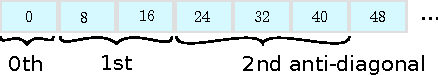
\includegraphics[scale=0.9]{figures/unaligned.pdf}
  \caption{Shift of the byte offset of the anti-diagonals}
  \label{fig:unaligned}
\end{figure}

Figure~\ref{fig:unaligned} shows how the byte offset for the anti-diagonals is shifted from one diagonal to the next {\bf to achieve a proper 16/32 byte alignment I assume?}.
To easily determine the aligned addresses for loading vectors we modified the indexing function {\bf TODO cross ref!} for the anti-diagonals. 
The main idea is to store each anti-diagonal starting at a 16/32 byte-aligned address. {\bf is the following edit I mad actually correct?} Thereby, all load and store operations are automatically correctly aligned.
%When iterating over anti-diagonal elements in a vectorized fashion, the vectors are then automatically constructed from data that is aligned to the required address offset.

{\bf The following three sentences need to be re-written, they are rather confusing} The starting address for the anti-diagonal is not the required alignment address for loading and storing the vectors, but a larger address minus the size of one double floating point value. 
This is due to the fact that the 0th row of the matrix is pre-computed during the matrix initialization and therefore a value is never written to this row. Another reason for this decision is that it is impossible to load all vectors needed for the computation inside the tight loop of the algorithm from an aligned addresses.

\begin{figure}[ht!]
  \centering
  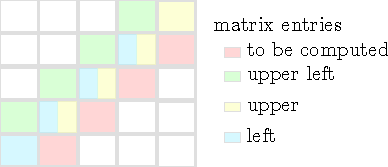
\includegraphics[scale=1.1]{figures/alignment.pdf}
  \caption{Outline of the data required for an operation in the DP loop}
  \label{fig:alignment}
\end{figure}

In Figure~\ref{fig:alignment}, we show the required values for computing the inner DP loop for AVX (vector length: $4$ double precision values). 
The elements marked in red are the ones we want to compute in the current step. 
For calculating a single element, we require three elements from the two previous columns. 
The element directly above (yellow) and left (blue) to the current element and the diagonal element above and to the left  (green) need to be loaded from the DP matrices. 
The Figure illustrates that (neglecting the asymptotically irrelevant boundary cases) one of the following four conditions holds:
\begin{enumerate}
  \item red and blue start on an aligned address, yellow and green do not
  \item red and yellow start on an aligned address, blue and green do not
  \item yellow and green start on an aligned address, red and blue do not
  \item red and green start on an aligned address, yellow and blue do not
\end{enumerate}

For the computation, we need to perform three \texttt{load} operations in total for the blue, yellow, and green elements and one \texttt{store} operation for the red elements. 
Since the {\em unaligned} \texttt{store} operation has greater relative performance impact than the unaligned load operations {\bf why?}, 
we ensured that either the first or the second of the above conditions is met. 
The first condition is implemented for the opening and middle part, the second condition holds true for the closing part of the DP matrices.

We achieved an appropriate alignment for each anti-diagonal by padding anti-diagonals as needed. 

% I think we don't need the stuff below. 
%We realized this padding by modifying the indexing function into the matrices. In the final version of this indexing function for an anti-diagonal, a certain amount of array elements in the matrix buffer is skipped. Elements are skipped until the second element of the anti-diagonal is aligned with the vector intrinsics requirements. This way, some memory is wasted because it is not used, however it is asymptotically insignificant compared to the overall space complexity of the algorithm ($O(\textrm{length}(\textrm{Sequence 1}) \cdot \textrm{length}(\textrm{Sequence 2}))$).

\section{Implementation of Team II}

In the following, we first describe how we transformed the algorithm into log-space to prevent numerical underflow. 
This also allowed us to simplify the formulas. 
Thereafter, we report how we improved data locality by storing the matrix entries in a dedicated data structure. 
While we experimented with different vectorization techniques, it turned out that the fastest code did not rely on vectorization. 
We thus conclude that, we managed to simplify the sequential code to such an extent, that, the potential advantages of using SIMD instructions 
are amortized by the additional overhead ({\bf TODO add cross-ref to the section where you discuss this}) we need for vectorization.

\subsection{Mathematical Optimization}

\subsubsection{Numerical Underflow Prevention}
\label{sec:log}

As the TKF91 algorithm performs successive multiplications on floating point numbers, preventing numerical underflow
{\em is} a major issue. Underflow can occur, even for short input sequences with less than $100$ nucleotides each.
To address this issue we transformed all computations into log-space, to add logarithms of probabilities instead of multiplying probabilities.
While it is still possible to experience under- or overflow {\bf why overflow, please explain!} even after this transformation, 
this is highly unlikely to occur for practical (empirical) input data.
We did not observe any numerical issues for the range of input parameters values and sequence lengths (up to and including $10000$ nucleotides) 
we tested.

\subsubsection{Simplifying the Formulas}  
We were able to omit redundant computations be re-using already computed values from previous matrix entries.
For example, we observed that $$M^0(i+1,0) = M^0(i,0) + \log(\gamma_{i+1}) + \log(\zeta_{i+1}) + \log(\beta(t)) + \log(\pi_{a_{i+1}}) + \log(\bar{p_0}(t)).$$
After replacing $\beta(t), \bar{p_0}(t), \gamma_i$ and $\zeta_i$ by their respective formulas, we observed that some terms appear multiple times. 
Operating in log-space allowed us to further simplify the formulas. Especially the logarithmic rules $\log(a*b) = \log(a) + \log(b)$ and $\log(a/b) = \log(a) - \log(b)$ 
allowed us to replace multiplications and divisions with additions and subtractions.
The resulting formulas can be found in Appendix~\ref{sec:formulas}. {\bf please include them here!}

\subsubsection{Pre-computing the Logarithms}
In general, replacing a multiplication by two logarithms and an addition is more costly. 
However, we managed to circumvent the additional computational cost of log space. 
This is because our formulas consist of sums of only $25$ different logarithms {\bf explain why this is the case} which we can simply 
pre-compute.

A major disadvantage of logarithmic transformations is that any error in the logarithm computation accumulates over a series of operations. 
To further investigate this, we used the high precision mathematical library of the \texttt{boost}-framework \cite{boost}. 
It offers datatypes that dynamically adapt their floating point precision to avoid numerical errors as well as under-/overflow. 
Our initial idea was to use this library only for pre-computing the logarithms, and thereby reduce the induced runtime overhead. 
However, transforming these arbitrary precision datatypes to standard double precision floating point values proved to be problematic, since 
it introduced additional loss of precision {\bf comapred to what?}. Therefore,  we abandoned this path.

\subsection{Matrix Storage Schemes}
\label{sec:caching}

\subsubsection{Matrix as Array}
In the first, na\"ive implementation, we stored each matrix ($M^0, M^1$, $M^2$) in a separate array, using row-major order. 
The matrix entry at position $(i,j)$ is stored at index position $i*(m+1)+j$ in the array (see Figure~\ref{fig:rowmajor}).

To illustrate the shortcomings of this approach, consider the following example: assume that six matrix rows fit into one cache line. 
Then, performing one iteration of the inner DP loop requires loading three cache lines, one per matrix. 
This is depicted in part a) of Figure~\ref{fig:cachelines}.
If we further assume a cache capacity of only two cache lines, 
every iteration would then force one of the lines to be swapped out, causing memory overhead.

\begin{figure}
\centering
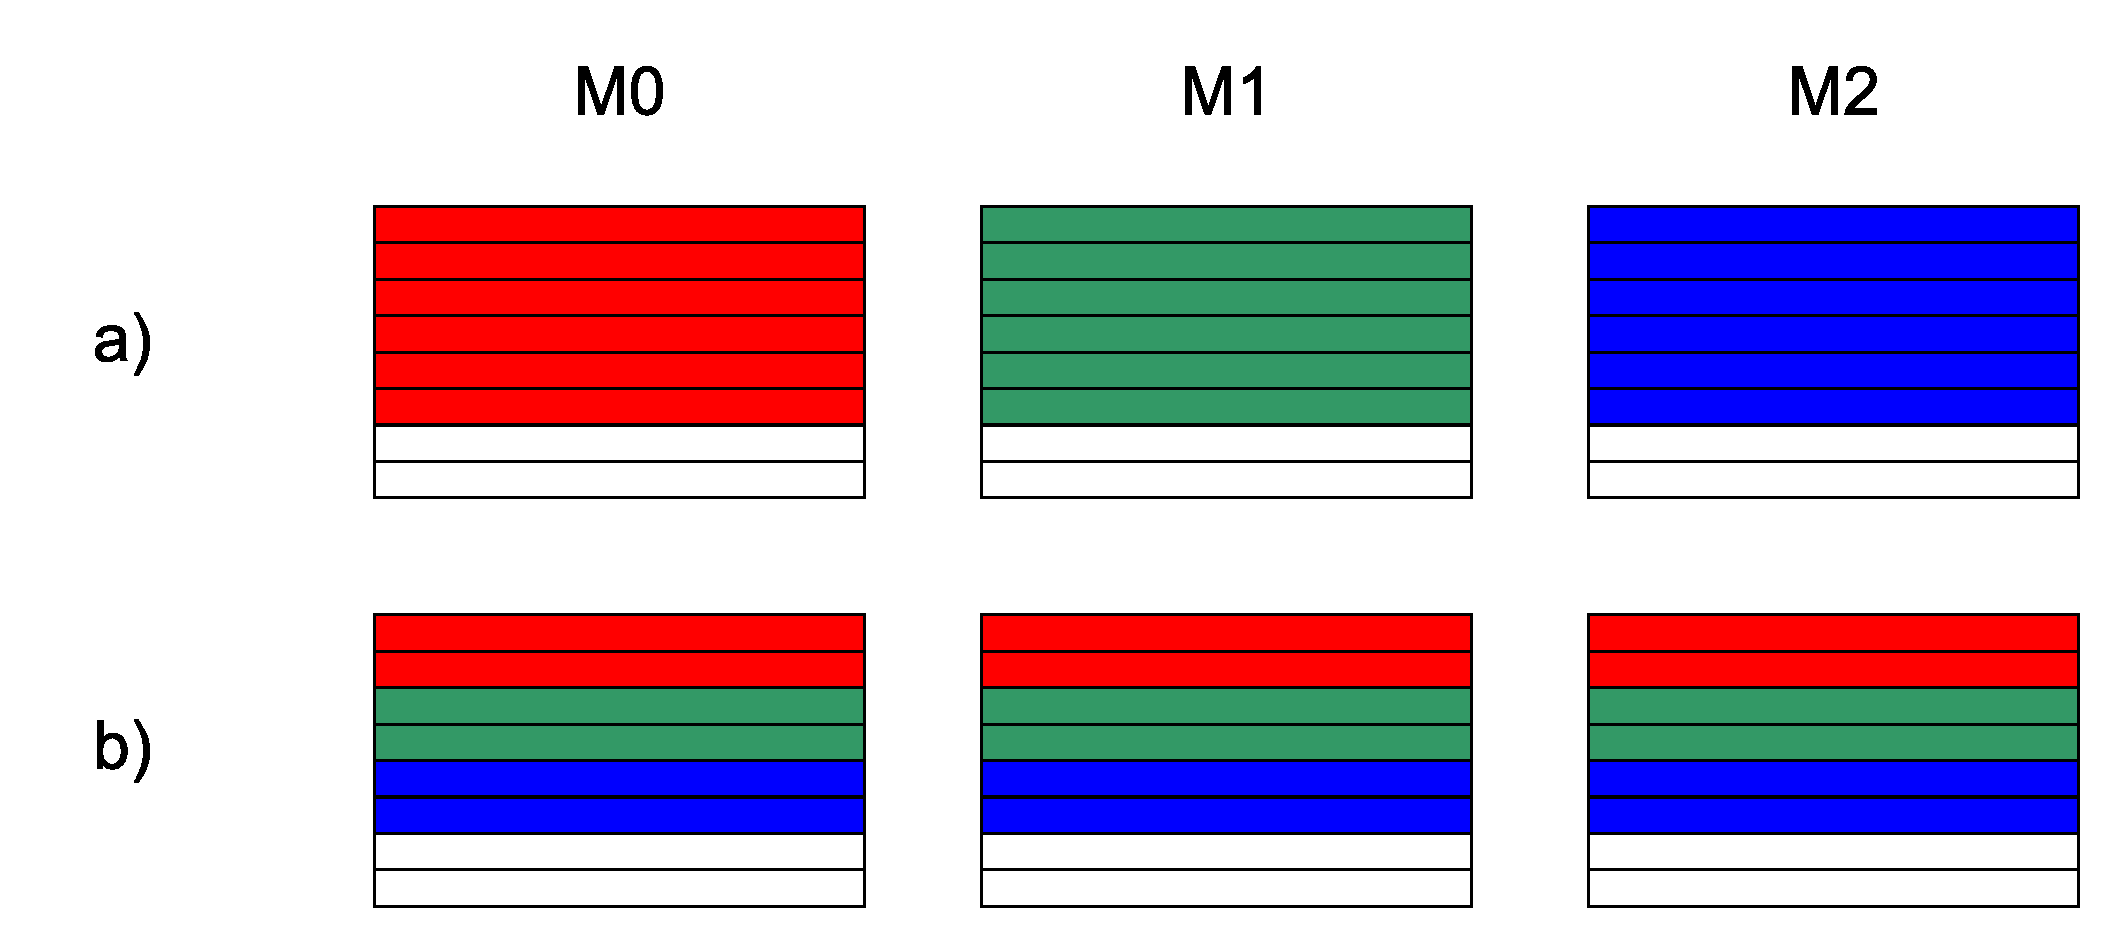
\includegraphics[width=\textwidth]{images/cachelines.pdf}
\caption{Relation of cache lines and matrices, using the method of allocating each matrix separately(\textbf{a)}) and the Array-of-Structs method (\textbf{b)}). 
Each color represents a distinct cache line.}
\label{fig:cachelines}
\end{figure}

\subsubsection{Array-of-Structs Data Structure}
The dynamic programming step (see Algorithm~\ref{alg:dp}) accesses the matrices $M^0, M^1$ and $M^2$ at the same index position to determine the maximum entry. 
Thus, we improved data locality by storing the entries from the three matrices at the same index position contiguously in memory. 
For this, we implemented a data structure called \texttt{MatrixEntry} that consists of three double values: \texttt{$m_0$}, \texttt{$m_1$} and \texttt{$m_2$}. 
Then, we used the Matrix as Array approach as before, but containing \texttt{MatrixEntry} structs as elements instead of simple 
\texttt{double} values (see Figure~\ref{fig:aos}). 

Let us now consider the example in Figure~\ref{fig:cachelines} again. 
With six matrix lines filling one cache line, a cache line now contains data from all three matrices. 
Consequently, all operations for a single computational iteration {\bf what do you mena by computational iteration?} 
will need to access two cache lines at most. 
If we assume a cache capacity of two cache lines again, cache misses will now only occur when traversing row boundaries.

By using the \texttt{perf stat} tool, we found that using the \texttt{MatrixEntry} data structure indeed reduced {\bf by how much, please quantify!} 
the number of page faults {\bf is this really called page faults? shouldn't it be cache misses?}.

\begin{algorithm}

\ldots\tcp{some initializations, see Appendix~\ref{sec:formulas:init}}
\For{$i = 1 , \ldots, n$} {
	\For{$j = 1, \ldots, m$} {
		\ldots\tcp{some initializations, see Appendix~\ref{sec:formulas:further}}
		
		$coord \gets CO(i, j)$\;	
		$up \gets CO(i, j-1)$\;
		$diag \gets CO(i-1, j-1)$\;		
		$left \gets CO(i-1, j)$\;
		
		$m[coord].m_0 \gets m[coord].m_0 + \max\{m[left].m_0, m[left].m_1, m[left].m_2\}$\;
		
		$m[coord].m_1 \gets m[coord].m_1 + \max\{m[diag].m_0, m[diag].m_1, m[diag].m_2\}$\;
		
		$m[coord].m_2 \gets m[coord].m_2 + \max\{m[up].m_1, m[up].m_2\}$\;
	}
}

\caption{The dynamic programming step, row-major version}
\label{alg:dp}
\end{algorithm}

\begin{figure}[width=\textwidth]
\centering
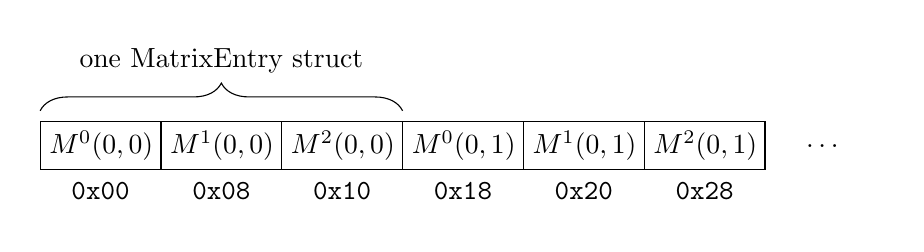
\begin{tikzpicture}[
    every node/.style={align=center, minimum height=1.5em, minimum width=1.5cm,node distance=0pt},
    background rectangle/.style={fill=black!0},show background rectangle, 
    ]
\node [cell](n1) at (0,0) {$M^0(0,0)$};
\node [cell, right = of n1] (n2) {$M^1(0,0)$};
\node [cell, right = of n2] (n3) {$M^2(0,0)$};
\node [cell, right = of n3] (n4) {$M^0(0,1)$};
\node [cell, right = of n4] (n5) {$M^1(0,1)$};
\node [cell, right = of n5] (n6) {$M^2(0,1)$};
\node [right = of n6](n7){\dots};
%\node [cell,right = of n7]{$M^2(n,m)$};

\node [below = of n1]{\texttt{0x00}};
\node [below = of n2]{\texttt{0x08}};
\node [below = of n3]{\texttt{0x10}};
\node [below = of n4]{\texttt{0x18}};
\node [below = of n5]{\texttt{0x20}};
\node [below = of n6]{\texttt{0x28}};

\draw[
   decorate,
  decoration={brace,amplitude=10pt}
]
  ([yshift=4pt]n1.north west) -- 
  node [black,yshift=18pt] {one MatrixEntry struct}
  ([yshift=4pt]n3.north east) ;

\end{tikzpicture}
\caption{Array-of-Structs data structure used to store the three matrices in memory. Each \texttt{MatrixEntry} elemnt stores 
the entries of a single coordinate for all three matrices. The structs are stored contiguously, as the figure depicts, in row-major order.}
\label{fig:aos}
\end{figure}


\subsubsection{Alternative Storage Schemes}
\label{par:otherattempts}
{\bf TODO: need to think how to match/connect this with the indexing that team I developed} 

Since each iteration in the dynamic programming step needs to access the top, left, and upper-diagonal elements of the matrices, 
a wave-front-like storage of the matrix (see Figure~\ref{fig:wavefront}) entries yields the lowest amount of expected cache misses. 
Finding an easy-to-compute {\bf do you mean easy or inexpensive?} closed formula that maps the index position $(i,j)$ representing the row and column of a matrix 
to wave-front-coordinates turned out to be challenging. 
The index of the diagonal is $i+j$, the sum of row index and column index. 
Determining the number of elements in the diagonal and especially the correct position within the diagonal proved more difficult though.
Since were not able to come up with an easy {\bf still not sure what you mean by easy} formula for the mapping, 
we tried storing pre-computed index mappings in an additional matrix. 
However, this slowed down the program as computing the mapped indices required more arithmetic operations than needed for the actual TKF algorithm.
Figure~\ref{fig:offset} illustrates the main problem which has to be solved 
for effective wave-front indexing effective: Given an wave-front index $k$, how do we obtain the indices for the upper, upper-left-diagonal and left element of the matrix? 
While the required offsets are constant within a {\bf anti?}diagonal, they change for different {\bf anti?}diagonals in the matrix.

\begin{figure}

\begin{minipage}{0.5\textwidth}
\centering
\begin{tabular}{|c|c|c|c|c|}
\hline 
0 & 1 & 2 & 3 & 4 \\ 
\hline 
5 & 6 & 7 & 8 & 9 \\ 
\hline 
10 & 11 & 12 & 13 & 14 \\ 
\hline 
15 & 16 & 17 & 18 & 19 \\ 
\hline
\end{tabular}
\caption{Row-major indexing}
\label{fig:rowmajor}
\end{minipage}
\begin{minipage}{0.5\textwidth}
\centering
\begin{tabular}{|c|c|c|c|c|}
\hline 
0 & 1 & 3 & 6 & 10 \\ 
\hline 
2 & 4 & 7 & 11 & 14 \\ 
\hline 
5 & 8 & 12 & 15 & 17 \\ 
\hline 
9 & 13 & 16 & 18 & 19 \\ 
\hline 
\end{tabular}
\caption{Wave-front indexing}
\label{fig:wavefront}
\end{minipage}
\end{figure}

\begin{figure}
\centering
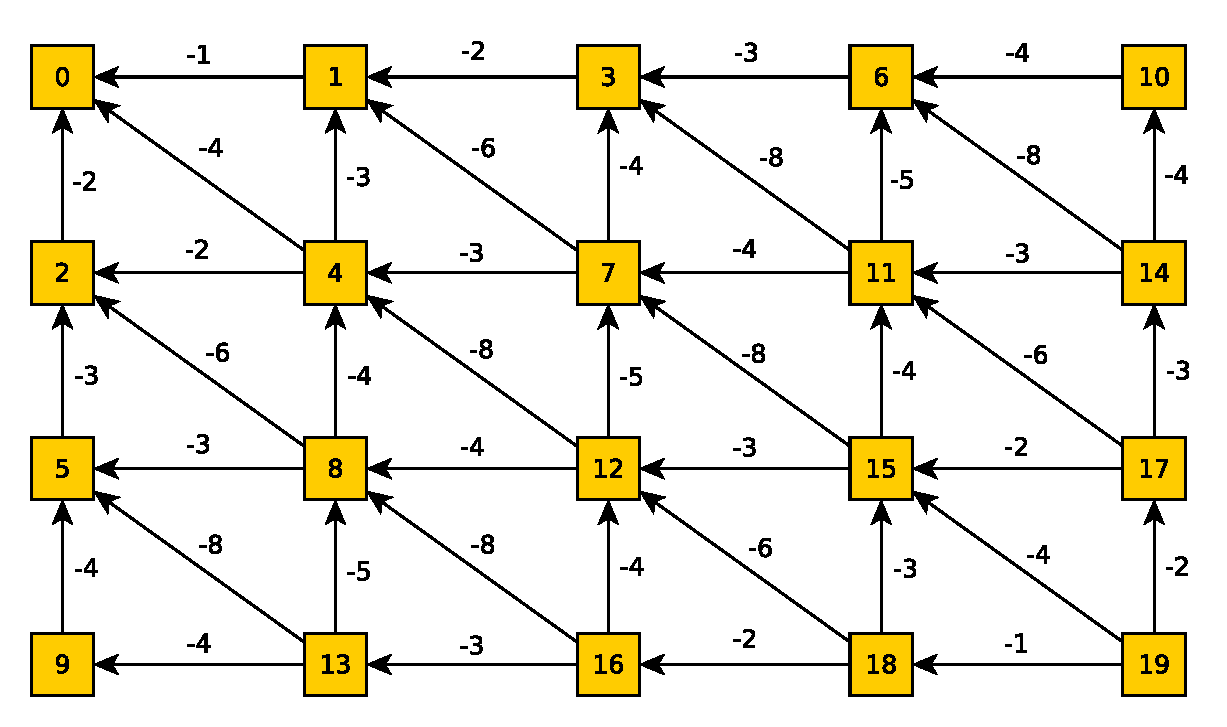
\includegraphics[scale=0.5]{images/unnamed0.pdf}
\caption{Offsets in wave-front indexing}
\label{fig:offset}
\end{figure}

%\section{Further Performance Tuning}
%- crlibm library
%- fixed-size array, no memset
%- store sequences as array of integers, used as a fast way to index precomputed logarithm values
%- fill matrices simultaneously (in the same loop)

\subsubsection{Vectorization Attempts}
\label{sec:vector}
During code development we conducted a partial vectorization for two of our implementations: 
the basic Log-space implementation (Section~\ref{sec:log}) and the improved Log-space implementation, using a more 
cache-efficient data structure to store the matrices (Section~\ref{sec:caching}).

In both cases we mainly focused on vectorizing the code that initializes the three matrices. 
This is because, our analyses with \texttt{Valgrind callgrind} revealed that this 
part of the code required $75-80\%$ of overall runtime. 
Additionally, as the initializations are completely independent of each other, this part should be straight-forward to vectorize.

Several code transformations were necessary to vectorize the code. 
First, we needed to guarantee that vector \texttt{load} and \texttt{store} operations are invoked on correctly aligned memory addresses. 
Secondly, we needed to devise a strategy for iterating over matrices and handling matrix sizes that are not multiples of the vector width.
Finally, we needed to store all calculation parameters {\bf what do you mean by calculation parameters?} in the appropriate vector types and 
had to replace all basic arithmetic operations by their vectorized counterparts.

\subsubsection{Log-space implementation}
For the vectorization of the basic {\bf did you properly introduce what the basic implementation is?} 
Log-space implementation we implemented appropriate memory alignment by using the \texttt{\_\_attribute\_\_(aligned(\textit{size}))} attribute for stack allocations, 
and the \texttt{posix\_memalign} function for heap allocations.

As a consequence, we also changed the iterations through the matrices to start at entry $0$ of each row, as starting iteration at position $1$ would result in incorrectly aligned memory accesses. 
Furthermore, as we stored the rows of the matrices contiguously in memory, we had to pad the row sizes 
to ensure the correct alignment of the first entry in each row.

The strategy we chose to deal with row dimensions that are not multiples of the vector width is straight forward. 
Per row, we compute as much as possible via vector intrinsics and the remainder sequentially. 

\subsubsection{Version using Array of Structs data structure}
While the strategy for dealing with row dimensions that do not fit vector widths remained the same in the improved version of our program, 
we had to apply several modifications to use vector intrinsics in conjunction with the more cache-efficient data structure.

As Figure~\ref{fig:aos} shows, using the Array-of-Structs scheme results in a non-contiguous storage of row entries. 
As a consequence, simply loading and storing vector registers cannot be used here. 
To this end, we implemented load and store operations that fit our data structure. These operations rely on vector functions that load and store single double precision floating point values. 
An advantage of this is that correct data alignment is not required any more. 
However, we believe {\bf why do you believe this, don't you have experimental evidence?} that this approach also induces a significant performance overhead 
compared to the classically used operations {\bf what are classically used operations?}.

\subsubsection{Thoughts on wave-front vectorization}
{\bf Maybe somehow make the wavefront parts more consistent to avoid redundnacies?} 
As the dynamic programming step of the TKF91 algorithm has data dependencies to the cells left of, above and diagonally left above of the cell to be computed, 
parallelization/vectorization requires a \textit{wave-front} approach.

In a wave-front parallelization, matrix entries are not computed by row or by column, but rather by computing the entries of each \textit{anti-diagonal} in parallel. 
Crucially, the individual anti-diagonals have to be computed sequentially and in-order when dependencies exist between subsequent anti-diagonals. 
In this case, the current anti-diagonal is the front of the wave traversing the DP matrix.

{\bf The following sentence is too long and confusing, please re-formulate!} As the log-space {\bf you use log-space inconssitently sometimes Log-spaca and sometimes as log-space} 
version of TKF91 reduces the operations that would require such a wave-front approach for parallelization to finding the greatest of two to three values, 
the relative amount of time spent doing so represents a negligible part of the overall algorithm. 
Nevertheless, we invested some time to devise a vectorized wave-front version of the program.

Initially, we attempted to find a suitable way for storing and accessing the matrix cells, 
to store data contiguously with respect to the wave-front data access pattern. 
We concluded that merely accessing {\bf accessing or indexing?} a cell, using the usual row-, and column coordinates, requires a significant amount of computation by itself. 
Most importantly, it {\bf what?} requires significantly more arithmetic operations {\bf please quantifdy!} than the actual computations conducted for each matrix entry.

Furthermore, our preliminary benchmarks had yielded absolutely no performance increase for the vectorized versions of either major implementation {\bf what are thos major im,plementations, maybe you 
should find better names for them}. 
As a consequence, we abandoned the wave-front vectorization approach.


\section{Evaluation and Testing}
\label{sec:evaluation}

\subsection{Benchmarks and Test Suites}
\label{ssec:benchmark}

An automated test suite is extremely valuable for re-factoring and optimizing the code, in that it provides the confidence of being able to detect regressions early and get helpful hints on how to fix them. We used the \textit{ctest} module of \textit{CMake} to invoke a Python script driving our console wrapper through a number of inputs. As we also used a continuous integration service running the tests on new commits, we could easily spot when a change accidentally broke the build. This development process lead to a high level of satisfaction and faith to try out different ideas in separate branches, while immediately getting feedback.

{\bf TODO consistency}

When the most obvious optimizations were done and we began to make use of vectorization instructions, we realized a benchmark suite based on the alignment data sets from the University of Oldenburg\footnote{http://goo.gl/nlD4nb} using the Celero C++ benchmarking library\footnote{https://github.com/DigitalInBlue/Celero} to have a reliable way of validating performance of our different approaches.

\subsection{Results of Team I}

From each of the six data sets, we picked ten nucleotide strings and computed all 45 pairwise alignments. We found that the median of five \textit{samples}, each of which consisting of the average of ten such \textit{iterations} (i.e. $5*10*45 = 2250$ alignments per data set) gave reliable performance estimates. As stated in Section~\ref{ssec:dataalignment}, we performed various performance comparisons based on this benchmark suite, such as the viability of different vector load and store schemes or the SoA, AoS, and AoSoA issue, of which the benchmark results on the reference hardware are depicted in Table~\ref{tbl:benchmark}. As already noted in Section~\ref{ssec:dataalignment}, we deemed the SoA approach the most performant.

\begin{table}[]
\centering
\label{tbl:benchmark}
\begin{tabular}{llll}
\begin{tabular}[c]{@{}l@{}}ms per iteration\\ (compared to best)\end{tabular} & SoA                & AoS                & AoSoA        \\
BDNF                                                                                      & 8.30 (1.01)        & {\bf 8.22 (1.00)}  & 8.51 (1.04)  \\
cytb                                                                                      & {\bf 26.19 (1.00)} & 29.07 (1.11)       & 29.65 (1.13) \\
RAG1                                                                                      & 20.88 (1.02)       & {\bf 20.56 (1.00)} & 20.94 (1.02) \\
RAG2                                                                                      & {\bf 24.64 (1.00)} & 25.09 (1.02)       & 25.83 (1.05) \\
RBP3                                                                                      & {\bf 35.26 (1.00)} & 36.35 (1.03)       & 37.62 (1.07) \\
vWF                                                                                       & 44.54 (1.01)       & {\bf 44.10 (1.00)} & 46.27 (1.05)
\end{tabular}
\caption{Benchmark results for SoA, AoS and AoSoA (from left to right)}
\end{table}

\subsection{Results of Team II}
{\bf TODO} 

We conducted all measurements on a desktop machine with $16$ GB RAM and
a Intel\texttrademark~i7-2600 CPU with $4$ physical cores and hyper-threading.

\subsection{Different Logarithm Libraries}
\label{sec:crlibm}

Additionally to using the \texttt{log} function from the standard C++ header \texttt{<math.h>}, we also used the \texttt{crlibm} library by Daramy et al.~\cite{Daramy04}. It includes versions of the natural logarithm computation, which allows the type of rounding to be explicitly specified.

In order to check the correctness of our resulting alignments, we computed the edit distance between the alignments we obtained by using different logarithm implementations. We assigned a cost of $1$ to insertions, deletions and substitutions of single letters. We picked all pairs of sequences from the \\ \texttt{BDNF\_unaligned\_sequences.fas} data set from \url{http://www.uni-oldenburg.de/fileadmin/user_upload/biologie/ag/systematik/download/Programs/benchMark_data.tar.gz}.

For the remaining parameters, we used $\lambda=1, \mu=2, \pi = (0.27, 0.24, 0.26,0.23)$ and $\tau = 0.1$. The edit distances were computed in relation to using the logarithm function from \texttt{Boost.Multiprecision}. 

In particular the \texttt{log\_ru} function, which explicitly rounds up, produces a notable change in alignment compared to the logarithm function from \\ \texttt{Boost.Multiprecision} as can be seen in Table~\ref{fig:dist}. The computed likelihood scores were highly similar and the differences in the alignments were minimal as can be seen in Figure~\ref{fig:alignments}. We finally decided to use the \texttt{log\_ru} function from the \texttt{crlibm} library because it had the most consent with the alignments returned by the reference implementation (\url{http://sco.h-its.org/exelixis/web/teaching/practical15/scaledCode/tkf91_scaling.tar.gz}).

\begin{table}[h!]

\centering

\begin{tabular}{|c|c|}
\hline 
Logarithm Function & Average Edit Distance \\ 
\hline 
\texttt{log} from \texttt{<math.h>} & 2.15 \\ 
\hline 
\texttt{log\_ru} from \texttt{crlibm} & 33.15 \\ 
\hline 
\end{tabular} 
\caption{Average edit distances from the alignment returned by using  \texttt{Boost.Multiprecision} of different logarithm implementations.}
\label{fig:dist}
\end{table}


\begin{figure}

\textbf{Alignment using standard C++ header \texttt{<math.h>}}
~
\\
\texttt{ACGACTAGTCA-GC-TACG-AT-CGA-CT-C-ATTCAACTGACTGACA-TCGACTTA} \\
\texttt{A-GAG-AGTAATGCATACGCATGC-ATCTGCTATT\textcolor{red}{\underline{---C}}TG-CTG-CAGTGG--T-A}
\\~\\
\textbf{Alignment using \texttt{Boost.Multiprecision}}
~
\\
\texttt{ACGACTAGTCA-GC-TACG-AT-CGA-CT-C-ATTCAACTGACTGACA-TCGACTTA} \\
\texttt{A-GAG-AGTAATGCATACGCATGC-ATCTGCTATT\textcolor{red}{\underline{---C}}TG-CTG-CAGTGG--T-A}
\\~\\
\textbf{Alignment using \texttt{log\_ru}}
~
\\
\texttt{ACGACTAGTCA-GC-TACG-AT-CGA-CT-C-ATTCAACTGACTGACA-TCGACTTA} \\
\texttt{A-GAG-AGTAATGCATACGCATGC-ATCTGCTATT\textcolor{red}{\underline{C---}}TG-CTG-CAGTGG--T-A}
\\~\\
\textbf{Alignment from reference implementation}
~
\\
\texttt{ACGACTAGTCA-GC-TACG-AT-CGA-CT-C-ATTCAACTGACTGACA-TCGACTTA} \\
\texttt{A-GAG-AGTAATGCATACGCATGC-ATCTGCTATT\textcolor{red}{\underline{C---}}TG-CTG-CAGTGG--T-A}

\caption{Difference in alignments using the input parameters $\pi=(0.25,0.25,0.25,0.25), \lambda=1, \mu = 2, \tau = 0.1$}
\label{fig:alignments}
\end{figure}

\subsection{Runtime Measurements}

The input sequences used to measure execution time were four pairs of randomly generated sequences of length $10$, $100$, $1000$ and $10000$ nucleotides. Sequences did not contain ambiguous characters. 

We measured the execution times around the kernel of the program, that is excluding any I/O required to load parameters and input sequences, or output of the algorithm. Kernel execution was performed multiple times per input and subsequently averaged. The number of runs executed was dependent on the size of the input, so as to balance accuracy and overall benchmark time (see Table~\ref{fig:runs}). 

\begin{table}
\centering

\begin{tabular}{|c|c|}
\hline 
Length of Sequence & Number of Runs \\ 
\hline 
$10$ & $10000$ \\ 
\hline 
$100$ & $1000$ \\ 
\hline 
$1000$ & $100$ \\ 
\hline 
$10000$ & $10$ \\ 
\hline 
\end{tabular}
\caption{Number of runs per sequence length}
\label{fig:runs}
\end{table}

\begin{figure}[h!]
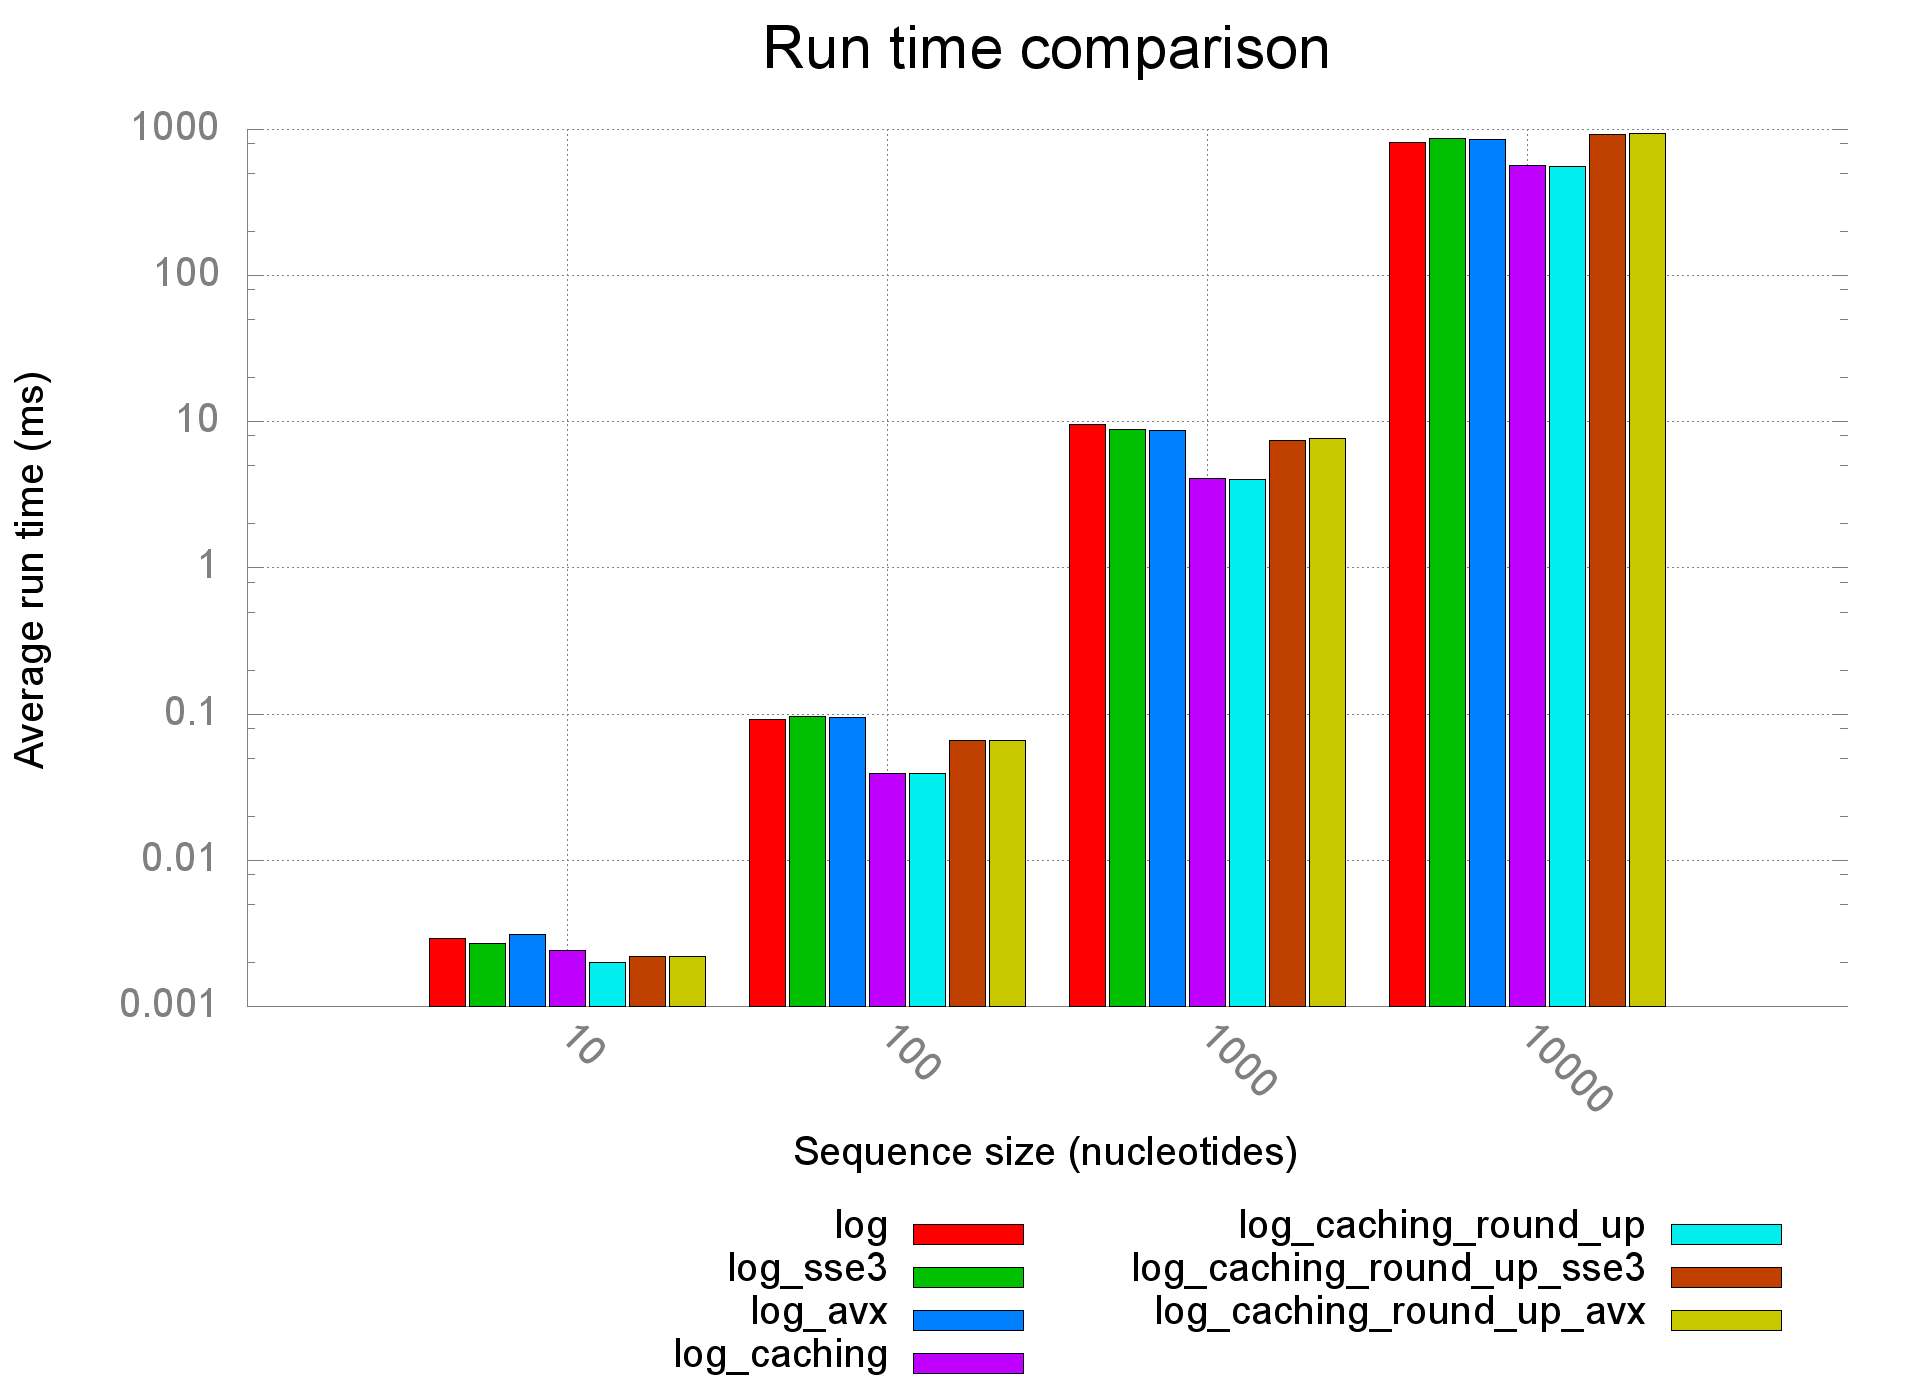
\includegraphics[width=\textwidth]{images/benchplot.png}
    \caption{Comparison of average run times of the different implementations. \texttt{sse3} and \texttt{avx} post-fixes denote the vectorized versions of the programs, using SSE3 and AVX vector intrinsics respectively (Section~\ref{sec:vector}). \texttt{log} denotes, that a version built on the log-space transformed version of TKF91 (Section~\ref{sec:log}). Versions using the Array-of-Structs method of storing matrices (Section~\ref{sec:caching}) are denoted by the \texttt{caching}-keyword, and the \texttt{round\_up}-keyword denotes the use of the \texttt{crlibm} library logarithm function \texttt{log\_ru} (Section~\ref{sec:crlibm}).}
\label{fig:runtime}
\end{figure}

\section{Teaching Results} 
\label{teaching-results} 
\subsection{What did Team I learn?}
While the assigned task was straightforward and very manageable in principle,
the implementation details were tricky.
Preventing floating point underflow while optimizing performance at the same time represented a challenge. 
This is because, such technical problems are frequently ignored in other programming practicals at KIT 
that emphasize functionality. 
Furthermore, vectorizing with SIMD intrinsics required some rethinking and re-engineering 
because we needed to identify a suitable memory layout, optimize data alignment, 
and deal with boundary conditions (padding). 
While it was satisfying to address and solve problems progressively, 
there were always additional ideas to further improve the code (w.r.t. performance and design), 
which made prioritizing tasks important.
We enjoyed the satisfaction of gaining yet another percent of execution time in combination 
with working with SIMD instructions that were not familiar to us.

The basic problem was clearly and outlined. There was enough freedom and time left 
to work on improving our solution. The scheduled project milestones 
turned procrastination and last minute work into a non-issue. 
Most surprisingly, we were always on schedule.

{\bf TODO: apart from SIMD were there any other new techniques or tools (e.g. cache analysis, clang compiler etc.) you used for the first time}

\subsection{What did Team II learn?}
For this assignment we had to tackle two major problems: preventing the loss of precision generated by numerical underflow and 
pursuing the elusive ``most efficient'' implementation. 
In the early stages, we came up with the idea of transforming the algorithm into log-space to solve the numerical issues. 
This did not only prove to represent an efficient solution, but also allowed us to further simplify the formulas and to pre-compute the vast majority of terms. 
In this context we also discovered deviations in the output alignments
that depend on the specific implementation of the logarithm function being used. 
We therefore used the \texttt{crlibm} library of mathematical functions, that allowed us to assess the impact of logarithm functions with distinct rounding strategies
on the final result.

To optimize the code we also used SSE3 and AVX intrinsics to vectorize the most work-intensive portions of the code. 
While we were unable to produce a faster vectorized code, we did learn how to use vector intrinsics and how to deal with the associated pitfalls. 
The largest performance gain was attained via a more cache-efficient data structure. 
For this, we used profiling tools such as \texttt{perf} and \texttt{valgrind cachegrind} for the first time {\bf correct?}. 
Finally,  we concluded that \verb|C++| is appropriate for HPC projects, provided that, the problem and data-structures at hand are well understood.

{\bf TODO: apart from SIMD were there any other new techniques or tools (e.g. cache analysis, clang compiler etc.) you used for the first time}

\subsection{What did the Teacher learn?}

{\bf TODO} 

\section{Conclusion}
\label{conclusion}
For other courses, integration, even faster codes, some of the techniques to be used for more complex stat aligners such as ....



%In this documentation we presented our implementation of the TKF91 evolutionary model for aligning sequences of DNA. Therefore we outlined the definition of an efficient memory layout, as well as measures to factor out complex computations during the tight loop in the DP algorithm. We presented our approach to the vectorization of the algorithm using SSE3 and AVX vector intrinsics and discussed how data can be efficiently aligned. Finally, the performance of the resulting application was tested and evaluated. 

%As a final note, we would like to remark that keeping the data spatially coherent by adjusting the memory layout through interleaving the matrices did not result in the performance gain that had first been anticipated. Unfortunately, the penalty of the shuffling and blending during loading and storing vectors, which has been introduced by those memory layouts, almost perfectly outweighed the gain in cache locality, which can be seen in Table~\ref{tbl:benchmark} in Section~\ref{sec:evaluation}.

\bibliographystyle{plain}
\bibliography{mlalign}

\end{document}
